
% LaTeX-Vorlage für Versuchsprotokolle
% Autor: Simon May
% Datum: 2017-10-05

% Es gibt die Dokumenttypen scrartcl („Artikel“), scrreprt („Bericht“),
% scrbook („Buch“) und scrlttr2 („Brief“). Diese gehören zum KOMA-Script,
% bieten mehr Optionen als die „Standardklassen“ und sollten besonders für
% deutsche Texte benutzt werden.
% Natürlich gibt es noch weitere Klassen, z.B. beamer für Präsentationen.
\documentclass[
	a4paper,                % Papierformat (DIN A4)
	titlepage=firstiscover, % Separate Titelseite
	captions=tableheading,  % \caption bei Tabellen immer als Überschrift setzen
	toc=bibliography,       % Literaturverzeichnis im Inhaltsverzeichnis aufführen
	toc=listof,             % Abbildungsverzeichnis etc. im Inhaltsverzeichnis aufführen
	oneside,                % Einseitig
	%twoside,               % Zweiseitig
	%twocolumn,             % Zweispaltig
	automark,               % Abschnittstitel automatisch in Kopfzeile einfügen
	12pt,                   % Schriftgröße (beliebige Größen mit „fontsize=Xpt“)
	english, ngerman,       % Sprache für z.B. Babel; ausgewählt: ngerman (letztgenannt)
	%draft=true             % Entwurf-Modus; markiert zu lange und zu kurze Zeilen
]{scrartcl}

% --- Pakete einbinden
% Autor: Simon May
% Datum: 2017-10-04

% --- Pakete einbinden
% --- Pakete erweitern LaTeX um zusätzliche Funktionen.
%     Dies ist ein Satz nützlicher Pakete.

% Silbentrennung etc.; Sprache wird durch Option bei \documentclass festgelegt
\usepackage{babel}
\usepackage{iftex}
\ifLuaTeX
	% Schriftart (Latin Modern)
	\usepackage{fontspec}
	\fontspec{Latin Modern Roman}
\else
	% Verwendung der Zeichentabelle T1 (für Sonderzeichen etc.)
	\usepackage[T1]{fontenc}
	% Legt die Eingabe-Zeichenkodierung fest, z.B. UTF-8
	\usepackage[utf8]{inputenc}
	% Schriftart (Latin Modern)
	\usepackage{lmodern}
	% Zusätzliche Sonderzeichen
	\usepackage{textcomp}
\fi

% Nutzen von +, -, *, / in \setlength u.ä. (z.B. \setlength{\a + 3cm})
\usepackage{calc}
% Wird benötigt, um \ifthenelse zu benutzen
\usepackage{xifthen}
% Optionen für eigene definierte Befehle
\usepackage{xparse}

% Verbessertes Aussehen des Schriftbilds durch kleine Anpassungen
\usepackage{microtype}
% Automatische Formatierung von Daten
\usepackage[useregional]{datetime2}
% Wird für Kopf- und Fußzeile benötigt
\usepackage{scrlayer-scrpage}
% Einfaches Wechseln zwischen unterschiedlichen Zeilenabständen
\usepackage{setspace}
% Optionen für Listen (enumerate, itemize, …)
\usepackage{enumitem}
% Automatische Anführungszeichen
\usepackage{csquotes}
% Zusätzliche Optionen für Tabellen (tabular)
\usepackage{array}

% Mathepaket (intlimits: Grenzen über/unter Integralzeichen)
\usepackage[intlimits]{amsmath}
% Mathe-Symbole, \mathbb etc.
\usepackage{amssymb}
% Weitere Mathebefehle
\usepackage{mathtools}
% „Schöne“ Brüche im Fließtext
\usepackage{xfrac}
% Ermöglicht die Nutzung von \SI{Zahl}{Einheit} u.a.
\usepackage{siunitx}
% Definition von Unicode-Symbolen; Nach [utf8]inputenc laden!
\usepackage{newunicodechar}
% Unicode-Formeln mit pdfLaTeX
% Autor: Simon May
% Datum: 2015-03-04

% Diese Datei ermöglicht es, Mathe-Symbole (z.B. \gamma) direkt als
% Sonderzeichen (d.h. γ) einzugeben

% silence unterdrückt Warnungen; vor hyperref laden
\usepackage{silence}
\WarningFilter[pdflatex-unicode-math]{newunicodechar}{Redefining Unicode character}
\ActivateWarningFilters[pdflatex-unicode-math]

\newunicodechar{†}{\dag}
\newunicodechar{‡}{\ddag}
\newunicodechar{…}{\ldots}
\newunicodechar{⋯}{\cdots}
\newunicodechar{⋮}{\vdots}
\newunicodechar{⋱}{\ddots}
\newunicodechar{⋰}{\iddots}
\newunicodechar{α}{\alpha}
\newunicodechar{β}{\beta}
\newunicodechar{γ}{\gamma}
\newunicodechar{δ}{\delta}
\newunicodechar{ε}{\varepsilon}
\newunicodechar{ϵ}{\epsilon}
\newunicodechar{ζ}{\zeta}
\newunicodechar{η}{\eta}
\newunicodechar{θ}{\theta}
\newunicodechar{ϑ}{\vartheta}
\newunicodechar{ι}{\iota}
\newunicodechar{κ}{\kappa}
\newunicodechar{ϰ}{\varkappa}
\newunicodechar{λ}{\lambda}
\newunicodechar{μ}{\mu}
\newunicodechar{ν}{\nu}
\newunicodechar{ξ}{\xi}
\newunicodechar{ο}{o}
\newunicodechar{π}{\pi}
\newunicodechar{ρ}{\rho}
\newunicodechar{ϱ}{\varrho}
\newunicodechar{σ}{\sigma}
\newunicodechar{τ}{\tau}
\newunicodechar{υ}{\upsilon}
\newunicodechar{φ}{\varphi}
\newunicodechar{ϕ}{\phi}
\newunicodechar{χ}{\chi}
\newunicodechar{ψ}{\psi}
\newunicodechar{ω}{\omega}
\newunicodechar{Α}{\mathrm{A}}
\newunicodechar{Β}{\mathrm{B}}
\newunicodechar{Γ}{\Gamma}
\newunicodechar{Δ}{\Delta}
\newunicodechar{Ε}{\mathrm{E}}
\newunicodechar{Ζ}{\mathrm{Z}}
\newunicodechar{Η}{\mathrm{H}}
\newunicodechar{Θ}{\Theta}
\newunicodechar{Ι}{\mathrm{I}}
\newunicodechar{Κ}{\mathrm{K}}
\newunicodechar{Λ}{\Lambda}
\newunicodechar{Μ}{\mathrm{M}}
\newunicodechar{Ν}{\mathrm{N}}
\newunicodechar{Ξ}{\Xi}
\newunicodechar{Ο}{\mathrm{O}}
\newunicodechar{Π}{\Pi}
\newunicodechar{Ρ}{\mathrm{P}}
\newunicodechar{Σ}{\Sigma}
\newunicodechar{Τ}{\mathrm{T}}
\newunicodechar{Υ}{\Upsilon}
\newunicodechar{Φ}{\Phi}
\newunicodechar{Χ}{\Chi}
\newunicodechar{Ψ}{\Psi}
\newunicodechar{Ω}{\Omega}
\newunicodechar{∑}{\sum}
\newunicodechar{∫}{\int}
\newunicodechar{∬}{\iint}
\newunicodechar{∭}{\iiint}
\newunicodechar{⨌}{\iiiint}
\newunicodechar{∮}{\oint}
\newunicodechar{∯}{\oiint}
\newunicodechar{∰}{\oiiint}
\newunicodechar{∇}{\nabla}
\newunicodechar{∂}{\partial}
\newunicodechar{√}{\sqrt}
\newunicodechar{∈}{\in}
\newunicodechar{∋}{\ni}
\newunicodechar{∉}{\notin}
\newunicodechar{∀}{\forall}
\newunicodechar{∃}{\exists}
\newunicodechar{∄}{\nexists}
\newunicodechar{∴}{\therefore}
\newunicodechar{∵}{\because}
\newunicodechar{〈}{\langle}
\newunicodechar{〉}{\rangle}
\newunicodechar{⌊}{\lfloor}
\newunicodechar{⌋}{\rfloor}
\newunicodechar{⌈}{\lceil}
\newunicodechar{⌉}{\rceil}
\newunicodechar{∼}{\sim}
\newunicodechar{∝}{\propto}
\newunicodechar{∞}{\infty}
\newunicodechar{ℵ}{\aleph}
\newunicodechar{ℏ}{\hbar}
\newunicodechar{℘}{\wp}
\newunicodechar{ℓ}{\ell}
\newunicodechar{∅}{\emptyset}
\newunicodechar{×}{\times}
\newunicodechar{⋅}{\cdot}
\newunicodechar{÷}{\div}
\newunicodechar{⋆}{\star}
\newunicodechar{∘}{\circ}
\newunicodechar{⋄}{\diamond}
\newunicodechar{⊕}{\oplus}
\newunicodechar{⊖}{\ominus}
\newunicodechar{⊗}{\otimes}
\newunicodechar{⊘}{\oslash}
\newunicodechar{⊙}{\odot}
\newunicodechar{±}{\pm}
\newunicodechar{∓}{\mp}
\newunicodechar{≈}{\approx}
\newunicodechar{≡}{\equiv}
\newunicodechar{≠}{\ne}
\newunicodechar{≥}{\ge}
\newunicodechar{≤}{\le}
\newunicodechar{≫}{\gg}
\newunicodechar{≪}{\ll}
\newunicodechar{⊂}{\subset}
\newunicodechar{⊃}{\supset}
\newunicodechar{⊆}{\subseteq}
\newunicodechar{⊇}{\supseteq}
\newunicodechar{⊈}{\nsubseteq}
\newunicodechar{⊉}{\nsupseteq}
\newunicodechar{≔}{\coloneqq}
\newunicodechar{≕}{\eqqcolon}
\newunicodechar{¬}{\neg}
\newunicodechar{∨}{\vee}
\newunicodechar{∧}{\wedge}
\newunicodechar{∪}{\cup}
\newunicodechar{∩}{\cap}
\newunicodechar{⋁}{\bigvee}
\newunicodechar{⋀}{\bigwedge}
\newunicodechar{⋃}{\bigcup}
\newunicodechar{⋂}{\bigcap}
\newunicodechar{⟂}{\perp}
\newunicodechar{∥}{\parallel}
\newunicodechar{∦}{\nparallel}
\newunicodechar{𝚤}{\imath}
\newunicodechar{𝚥}{\jmath}
\newunicodechar{⇔}{\Leftrightarrow}
\newunicodechar{⇕}{\Updownarrow}
\newunicodechar{⇐}{\Leftarrow}
\newunicodechar{⇒}{\Rightarrow}
\newunicodechar{⇑}{\Uparrow}
\newunicodechar{⇓}{\Downarrow}
\newunicodechar{↔}{\leftrightarrow}
\newunicodechar{↕}{\updownarrow}
\newunicodechar{←}{\leftarrow}
\newunicodechar{→}{\rightarrow}
\newunicodechar{↑}{\uparrow}
\newunicodechar{↓}{\downarrow}
\newunicodechar{⟷}{\longleftrightarrow}
\newunicodechar{⟵}{\longleftarrow}
\newunicodechar{⟶}{\longrightarrow}
\newunicodechar{⇇}{\leftleftarrows}
\newunicodechar{⇉}{\rightrightarrows}
\newunicodechar{⇈}{\upuparrows}
\newunicodechar{⇊}{\downdownarrows}
\newunicodechar{⟺}{\Longleftrightarrow}
\newunicodechar{⟸}{\Longleftarrow}
\newunicodechar{⟹}{\Longrightarrow}
\newunicodechar{↦}{\mapsto}
\newunicodechar{↤}{\mapsfrom}
\newunicodechar{⟼}{\longmapsto}
\newunicodechar{⟻}{\longmapsfrom}
\newunicodechar{⟾}{\Longmapsto}
\newunicodechar{⟽}{\Longmapsfrom}
\newunicodechar{↗}{\nearrow}
\newunicodechar{↖}{\nwarrow}
\newunicodechar{↘}{\searrow}
\newunicodechar{↙}{\swarrow}
\newunicodechar{↩}{\hookleftarrow}
\newunicodechar{↪}{\hookrightarrow}
\newunicodechar{↶}{\curvearrowleft}
\newunicodechar{↷}{\curvearrowright}
\newunicodechar{↺}{\circlearrowleft}
\newunicodechar{↻}{\circlearrowright}
\newunicodechar{↫}{\looparrowleft}
\newunicodechar{↬}{\looparrowright}
\newunicodechar{⇋}{\leftrightharpoons}
\newunicodechar{⇌}{\rightleftharpoons}
\newunicodechar{↼}{\leftharpoonup}
\newunicodechar{↽}{\leftharpoondown}
\newunicodechar{⇀}{\rightharpoonup}
\newunicodechar{⇁}{\rightharpoondown}
\newunicodechar{↿}{\upharpoonleft}
\newunicodechar{↾}{\upharpoonright}
\newunicodechar{⇃}{\downharpoonleft}
\newunicodechar{⇂}{\downharpoonright}
\newunicodechar{𝔸}{\mathbb{A}}
\newunicodechar{𝔹}{\mathbb{B}}
\newunicodechar{ℂ}{\mathbb{C}}
\newunicodechar{𝔻}{\mathbb{D}}
\newunicodechar{𝔼}{\mathbb{E}}
\newunicodechar{𝔽}{\mathbb{F}}
\newunicodechar{𝔾}{\mathbb{G}}
\newunicodechar{ℍ}{\mathbb{H}}
\newunicodechar{𝕀}{\mathbb{I}}
\newunicodechar{𝕁}{\mathbb{J}}
\newunicodechar{𝕂}{\mathbb{K}}
\newunicodechar{𝕃}{\mathbb{L}}
\newunicodechar{𝕄}{\mathbb{M}}
\newunicodechar{ℕ}{\mathbb{N}}
\newunicodechar{𝕆}{\mathbb{O}}
\newunicodechar{ℙ}{\mathbb{P}}
\newunicodechar{ℚ}{\mathbb{Q}}
\newunicodechar{ℝ}{\mathbb{R}}
\newunicodechar{𝕊}{\mathbb{S}}
\newunicodechar{𝕋}{\mathbb{T}}
\newunicodechar{𝕌}{\mathbb{U}}
\newunicodechar{𝕍}{\mathbb{V}}
\newunicodechar{𝕎}{\mathbb{W}}
\newunicodechar{𝕏}{\mathbb{X}}
\newunicodechar{𝕐}{\mathbb{Y}}
\newunicodechar{ℤ}{\mathbb{Z}}
\newunicodechar{𝒜}{\mathcal{A}}
\newunicodechar{ℬ}{\mathcal{B}}
\newunicodechar{𝒞}{\mathcal{C}}
\newunicodechar{𝒟}{\mathcal{D}}
\newunicodechar{ℰ}{\mathcal{E}}
\newunicodechar{ℱ}{\mathcal{F}}
\newunicodechar{𝒢}{\mathcal{G}}
\newunicodechar{ℋ}{\mathcal{H}}
\newunicodechar{ℐ}{\mathcal{I}}
\newunicodechar{𝒥}{\mathcal{J}}
\newunicodechar{𝒦}{\mathcal{K}}
\newunicodechar{ℒ}{\mathcal{L}}
\newunicodechar{ℳ}{\mathcal{M}}
\newunicodechar{𝒩}{\mathcal{N}}
\newunicodechar{𝒪}{\mathcal{O}}
\newunicodechar{𝒫}{\mathcal{P}}
\newunicodechar{𝒬}{\mathcal{Q}}
\newunicodechar{ℛ}{\mathcal{R}}
\newunicodechar{𝒮}{\mathcal{S}}
\newunicodechar{𝒯}{\mathcal{T}}
\newunicodechar{𝒰}{\mathcal{U}}
\newunicodechar{𝒱}{\mathcal{V}}
\newunicodechar{𝒲}{\mathcal{W}}
\newunicodechar{𝒳}{\mathcal{X}}
\newunicodechar{𝒴}{\mathcal{Y}}
\newunicodechar{𝒵}{\mathcal{Z}}
\newunicodechar{𝕬}{\mathfrak{A}}
\newunicodechar{𝕭}{\mathfrak{B}}
\newunicodechar{𝕮}{\mathfrak{C}}
\newunicodechar{𝕯}{\mathfrak{D}}
\newunicodechar{𝕰}{\mathfrak{E}}
\newunicodechar{𝕱}{\mathfrak{F}}
\newunicodechar{𝕲}{\mathfrak{G}}
\newunicodechar{𝕳}{\mathfrak{H}}
\newunicodechar{𝕴}{\mathfrak{I}}
\newunicodechar{𝕵}{\mathfrak{J}}
\newunicodechar{𝕶}{\mathfrak{K}}
\newunicodechar{𝕷}{\mathfrak{L}}
\newunicodechar{𝕸}{\mathfrak{M}}
\newunicodechar{𝕹}{\mathfrak{N}}
\newunicodechar{𝕺}{\mathfrak{O}}
\newunicodechar{𝕻}{\mathfrak{P}}
\newunicodechar{𝕼}{\mathfrak{Q}}
\newunicodechar{𝕽}{\mathfrak{R}}
\newunicodechar{𝕾}{\mathfrak{S}}
\newunicodechar{𝕿}{\mathfrak{T}}
\newunicodechar{𝖀}{\mathfrak{U}}
\newunicodechar{𝖁}{\mathfrak{V}}
\newunicodechar{𝖂}{\mathfrak{W}}
\newunicodechar{𝖃}{\mathfrak{X}}
\newunicodechar{𝖄}{\mathfrak{Y}}
\newunicodechar{𝖅}{\mathfrak{Z}}

\DeactivateWarningFilters[pdflatex-unicode-math]


% Farben
\usepackage{xcolor}
% Einbinden von Grafiken (\includegraphics)
\usepackage{graphicx}
% .tex-Dateien mit \includegraphics einbinden
\usepackage{gincltex}
% Größere Freiheiten bei Dateinamen mit \includegraphics
\usepackage{grffile}
% Abbildungen im Fließtext
\usepackage{wrapfig}
% Zitieren, Bibliographie (Biber als Bibliographie-Programm verwenden!)
\usepackage[style=verbose, backend=biber]{biblatex}
% Abbildungen nebeneinander (subfigure, subtable)
\usepackage{subcaption}

% Verlinkt Textstellen im PDF-Dokument (sollte am Ende geladen werden)
\usepackage[unicode]{hyperref}
% „Schlaue“ Referenzen (nach hyperref laden!)
\usepackage{cleveref}
%PDF einbinden
%\usepackage{pdfpages}
%Graphiken zeichnen
%\usepackage{tikz}
%\usetikzlibrary{angles,quotes,babel,3d}
% --- Einstellungen
% -- LaTeX/KOMA
% 1,5-facher Zeilenabstand
\onehalfspacing
\recalctypearea
% Schrift bei Bildunterschriften ändern
\addtokomafont{caption}{\small}
\addtokomafont{captionlabel}{\bfseries}
% Nummerierung der Formeln entsprechend des Abschnitts (z.B. 1.1)
\numberwithin{equation}{section}
% „Verwaiste“ Zeilen am Seitenanfang/-Ende stärker vermeiden
\clubpenalty=1000
\widowpenalty=1000
% Auf mehrere Seiten aufgespaltene Fußnoten stärker vermeiden
\interfootnotelinepenalty=3000

% -- csquotes
% Anführungszeichen automatisch umwandeln
\MakeOuterQuote{"}

% -- siunitx
\sisetup{
	locale=DE,
	separate-uncertainty,
	output-product=\cdot,
	quotient-mode=fraction,
	per-mode=fraction,
	fraction-function=\sfrac
}

% -- hyperref
\hypersetup{
	% Links/Verweise mit Kasten der Dicke 0.5pt versehen
	pdfborder={0 0 0.5}
}

% -- cleveref
\crefname{equation}{}{}
\Crefname{equation}{}{}

% -- biblatex (Literaturverzeichnis)
\IfFileExists{res/literatur.bib}{
	\addbibresource{res/literatur.bib}
}{}

\AtEndPreamble{
	% Kopf- und Fußzeile konfigurieren
	\ifthenelse{\boolean{showHeader}}{
		\KOMAoptions{headsepline}
		\recalctypearea
		\automark{section}
		% Innenseite der Kopfzeile
		\ihead{\headmark}
		% Mitte der Kopfzeile
		\chead{}
		% Außenseite der Kopfzeile
		\ohead{\usekomafont{pagehead}\varAutor}
	}{}
	% Innnenseite der Fußzeile
	\ifoot{}
	% Mitte der Fußzeile          
	\cfoot{-~\pagemark~-}
	% Außenseite der Fußzeile
	\ofoot{}

	% Metadaten für die PDF-Datei
	\hypersetup{
		pdftitle={Versuchsprotokoll: \varName},
		pdfauthor={\varAutor},
		pdfsubject={Grundpraktikum},
		pdfkeywords={Physik, Münster, Praktikum, Versuchsprotokoll}
	}
}



% --- Eigene Befehle einbinden
% Autor: Simon May
% Datum: 2017-10-05

% Eigene Befehle eignen sich gut, um Abkürzungen für lange Befehle zu erstellen.
% So vermeidet man, dass man immer wieder dasselbe Konstrukt kopieren und
% einfügen muss und, wenn man dann doch etwas ändern will, an zahllosen Stellen
% im Dokument dieselbe Änderung vornehmen muss.
% Die Syntax ist die folgende:
% \newcommand{neuer Befahl}[Anzahl Parameter (optional)]{Inhalt}
% Das folgende Beispiel fügt ein Bild mit bestimmten vorgegebenen Optionen ein:
\newcommand{\centeredImage}[1]{
	\begin{figure}
		\centering
		\includegraphics[width=0.5\textwidth]{#1}
	\end{figure}
}
% #1 ist dabei ein Parameter, den man \centeredImage übergeben muss, also:
% \centeredImage{...}
% Benötigt man keine Parameter, dann lässt man [1] weg. Werden zusätzliche
% Parameter benötigt, dann kann man die Zahl auf maximal 9 erhöhen.

% Ein Befehl, um eine E-Mail-Adresse darzustellen bzw. automatisch zu verlinken
\newcommand{\email}[1]{\href{mailto:#1}{\texttt{#1}}}

% \arsinh etc.
\newcommand*{\arsinh}{\operatorname{arsinh}}
\newcommand*{\arcosh}{\operatorname{arcosh}}
\newcommand*{\artanh}{\operatorname{artanh}}
\newcommand*{\const}{\text{const.}}


% --- Variablen importieren
% Autor: Simon May
% Datum: 2016-10-13
% Der Befehl \newcommand kann auch benutzt werden, um „Variablen“ zu definieren:

% Nummer laut Praktikumsheft:
\newcommand*{\varNum}{M3}
% Name laut Praktikumsheft:
\newcommand*{\varName}{Elastizität}
% Datum der Durchführung (Format: JJJJ-MM-TT):
\newcommand*{\varDatum}{2017-12-00}
% Autoren des Protokolls:
\newcommand*{\varAutor}{Hauke Hawighorst, Jörn Sieveneck}
% Nummer der eigenen Gruppe:
\newcommand*{\varGruppe}{Gruppe 9}
% E-Mail-Adressen der Autoren (kommagetrennt ohne Leerzeichen!):
\newcommand{\varEmail}{h.hawighorst@uni-muenster.de,j\_siev11@uni-muenster.de}
%betreuer Name
\newcommand{\varBetreuer}{\normalsize betreut von \\ Christian Thiede  }
% E-Mail-Adresse anzeigen (true/false):
\newcommand*{\varZeigeEmail}{true}
% Kopfzeile anzeigen (true/false):
\newcommand*{\varZeigeKopfzeile}{true}
% Inhaltsverzeichnis anzeigen (true/false):
\newcommand*{\varZeigeInhaltsverzeichnis}{true}
% Literaturverzeichnis anzeigen (true/false):
\newcommand*{\varZeigeLiteraturverzeichnis}{true}


\newboolean{showEmail}
\setboolean{showEmail}{\varZeigeEmail}
\newboolean{showHeader}
\setboolean{showHeader}{\varZeigeKopfzeile}
\newboolean{showTOC}
\setboolean{showTOC}{\varZeigeInhaltsverzeichnis}
\newboolean{showBibliography}
\setboolean{showBibliography}{\varZeigeLiteraturverzeichnis}

\begin{document}

% Römische Seitenzahlen für Titelseite/Inhaltsverzeichnis
\pagenumbering{roman}
% Zunächst ohne Kopf-/Fußzeile
\pagestyle{scrplain}

% --- Titelseite einbinden
%     Falls die Datei „res/titelbild.pdf“ existiert, wird sie auf der Titelseite
%     eingefügt
\IfFileExists{tex/04_Titelseite.tex}{
	% Autor: Simon May
% Datum: 2017-10-05

% Befehl, um die E-Mail-Adressen auf der Titelseite darzustellen
\makeatletter
\newcommand*{\protokollemailparse}[1]{%
	\@for\@tempa:=#1\do{%
		\normalsize\email{\@tempa}\\
	}%
}
\makeatother

\title{Versuchsprotokoll \varNum}
\subtitle{\varName}
\subject{Experimentelle Übungen~I}
\date{\DTMdate{\varDatum}}
\ifthenelse{\boolean{showEmail}}{%
	\author{\varAutor\\\normalsize\varGruppe\\\protokollemailparse{\varEmail} \\ \varBetreuer}%
}{%
	\author{\varAutor\\\normalsize\varGruppe \\ \varBetreuer}%
}




% Falls die Datei „res/titelbild.pdf“ existiert, wird sie hier eingefügt
\IfFileExists{res/titelbild.pdf}{
	\publishers{\vspace{2ex}\includegraphics[width=0.75\textwidth]{res/titelbild.pdf}}
}{}

\maketitle

}{}

% --- Inhaltsverzeichnis einbinden
\ifthenelse{\boolean{showTOC}}{
	\tableofcontents
	\clearpage
}{}

% Zurücksetzen der Seitenzahlen auf arabische Ziffern
\pagenumbering{arabic}
% Ab hier mit Kopf- und Fußzeile
\pagestyle{scrheadings}

% --- Den Inhalt der Arbeit einbinden
%Zusammenfassung in unter 200 Wörtern

\section{Zusammenfassung}\label{kap:Zusammenfassung}

Der Versuchtag bestand aus zwei Experimenten welche die Rotation starrer Körper betrachten, zunächst wurde das Fallverhalten des Maxwellsche Fallrad, ähnlich einem Jo-Jo, untersucht und anschließend die Präzessionsbewegung eines Kreisels. 



%Fallrad


Das Maxwellsche Fallrad eignet sich zur Untersuchung von gleichmäßig beschleunigten Bewegungen, da die potentielle Energie in Translation und Rotation umgewandelt wird somit hat das Rad eine geringere Geschwindigkeit und die Bewegung lässt sich ohne aufwendige Messinstrumente beobachten, da die Fallzeiten groß genug waren um sie mit einer Herkömmlichen Stoppuhr zu messen.
Aus Abmessungen und Gewicht wurde das Trägheitsmoment bezüglich der Symmetrieachse $J_s=\SI{0.003702 \pm 0.000008}{kg\cdot m^2}$ bestimmt, anschließend wurde aus den Fallzeiten die effektive Beschleunigung  $g^*=\SI{0.0410 \pm  0.0019}{m \per s \squared}$ bestimmt. Abschließend wurde mit dem Steinerschen Satz auf den Abrollradius $R=\SI{0.00460\pm 0.00011}{m}$ geschlossen und mit dem gemessenen Abrollradius $R_{geometrisch}=\SI{0.00455 \pm 0.00004}{m}$ verglichen. Der geometrisch bestimmte Wert bestätigt die vorherige Messung. 






 

%Kreisel

Im zweiten Experiment wurde die Präzessionszeit $T_p$ eines Kreisels bei einer annähernd Konstanten Winkelgeschwindigkeit $\omega$. Bei dem Untersuchten Kreisel handelte es sich um einen Schweren Symmetrischen Kreisel.
Durch das Experiment sollte das Trägheitsmoment J des Kreisels Bestimmt werden. Einmal experimentell über den Zusammenhang zwischen $\frac{\Delta \omega}{\Delta T_p}$ und dem Produkt aus der Kraft F und dem Abstand l zwischen dem Unterstützungspunkt und dem Angriffspunkt des Kraftmessers vgl. Abb. \ref{fig:Kreisel}(im folgendem $J_{exp.}$ genannt). Und einmal aus der Masse und dem Radius der Kugel sowie einem gegebenen Trägheitsmoment des Stabes mit dem Zusatzgewicht im folgendem $J_{theo}$ genannt. Da sich $J_{theo.}=\SI{1,3356+-0,0004e-4}{kg \cdot m^2}$ und $J_{exp.}=\SI{1,0194+-0,0319e-4}{kg \cdot m^2}$ deutlich von einander Unterscheiden ist vermutlich darauf zurückzuführen das beim experimentieren Fehler unterlaufen sind.  
 














\section{Innenwiederstand einer Batterie}

Es sollte der Innenwiederstand einer Schaltung aus Akkumulatoren bestimmt werden. Zur Verdeutlichung des Effektes wurde vor jeden Akkumulator ein Widerstand geschaltet. 

\subsection{Methoden}


Zur Bestimmung des Innenwiederstandes wurde die Klemmspannung der Spannungsquelle für verschiedene Außenwiderstände gemessen. Aus Spannung und Widerstand wurden die Spannung $U$ in Abhängigkeit der Stromstärke $I$ (\cref{fig:batt-ges-u}) und die Leistung $P$ in Abhängigkeit des Außenwiederstandes $R_a$ (\cref{fig:batt-ges-p}) berechnet. Aus den Ausgleichskurven folgen jeweils die Klemmspannung ohne Last $U_0$ sowie der Innenwiederstand $R_i$. Betrachtet wurden als Spannungsquelle: eine einzelne Monozelle, eine Parallelschaltung sowie eine Reihenschaltung aus drei Monozellen. 

Aus der Ableseungenauigkeit des Voltmeters folgt als Standardunsicherheit u(U)=\SI{0.2}{V}, die relative Unsicherheit der Steckwiederstände wurde mit 5\% abgeschätzt.





\subsection{Daten und Analyse}


Aus den Messpunkten $U(R_a)$ folgt mit dem Ohmschen Gesetz \cref{fig:batt-ges-u}. Aus $U_{Kl}=U_0-R_a I$ folgt, dass die Steigung des Ausgleichsgerade dem negativen des Innenwiderstandes entspricht. Ohne Stromfluss gilt $U_0=U_{Kl}$, deswegen entspricht der Y-Achsenabschnitt der Leerlaufspannung $U_0$ der "idealen Spannungsquelle" \cite{lw}. Die aus den Parametern der Anpassungsgerade gefundenen Werte sind in \cref{tab:batt-U-R} dargestellt.





\begin{table}
	\caption{Leerlaufspannung und Innenwiderstand der Spannungsquellen aus den Kennlinien}
	\centering
	\begin{tabular}{|l l||c|c|}
		\hline 
		Schaltung & Index	& Leerlaufspannung $U_0$ & Innenwiederstand $R_i$ \\ 
		\hline \hline
		Einzelne Monozelle	&E& \SI{1.28+-0.01}{V}  & \SI{17.7+-0.4}{\ohm } \\ 
		\hline  
		Parrallelschaltung	&P& \SI{1.289+-0.003}{V } &\SI{5.99+-0.06}{\ohm }  \\ 
		\hline   
		Reihenschaltung	&R& \SI{4.03+-0.12}{V } &\SI{57+-3}{\ohm }  \\ 
		\hline 
	\end{tabular} 
	
	\label{tab:batt-U-R}
	
\end{table}


 


\begin{figure}[h]
	\centering
	\includegraphics[width=0.9\linewidth]{"auswertung/Auswertung Innenwiderstand/Batterie Gesamt U"}
	\caption{Spannungsverläufe der Monozelle~$U_E$, der Parallelschaltung von drei Monozellen~$U_P$ und der Reihenschaltung von drei Monozellen~$U_R$ in Abhängigkeit der Stromstärke~$I$.}
	\label{fig:batt-ges-u}
\end{figure}










\FloatBarrier
%Leistung

\begin{figure}[h]
	\centering
	\includegraphics[width=0.9\linewidth]{"auswertung/Auswertung Innenwiderstand/Batterie Gesamt P"}
	\caption{Leistung $P$ am Lastwiderstand $R_a$ in dessen Abhängigkeit}
	\label{fig:batt-ges-p}
\end{figure}



\begin{table}
	\caption{Leerlaufspannung und Innenwiderstand der Spannungsquellen aus der Leistung}
	\centering
	\begin{tabular}{|l l||c|c|}
		\hline 
		Schaltung & Index	& Leerlaufspannung $U_0$ & Innenwiederstand $R_i$ \\ 
		\hline \hline
		Einzelne Monozelle	&E& \SI{1.27+-0.02}{V}  & \SI{17.6+-0.6}{\ohm } \\ 
		\hline  
		Parrallelschaltung	&P& \SI{1.282+-0.007}{V } &\SI{5.91+-0.09}{\ohm }  \\ 
		\hline   
		Reihenschaltung	&R& \SI{4.26+-0.21}{V } &\SI{63+-5}{\ohm }  \\ 
		\hline 
	\end{tabular} 
	
	\label{tab:batt-U-P}
	
\end{table}


%In analoger Weise zu \cref{fig:batt-ges-u} wurde \cref{fig:batt-ges-p} erstellt. 
Die Leistung am äußeren Widerstand ist gegeben durch 
\begin{align}
 P &=\frac{U_{Kl}^2}{R_a} \label{eq:puk}\\
 &= U_0^2 \frac{R_a}{(R_a+R_i)^2} \label{eq:pu0}.
\end{align} 
Gleichung~\ref{eq:puk} wurde verwendet um die Leistungen zu berechnen, die Ausgleichskurve wurde nach Gleichung~\ref{eq:pu0} erstellt.
Die Werte für $U_0$ und $R_i$ ergeben sich aus der Ausgleichskurve und sind in \cref{tab:batt-U-P} dargestellt. Die Maximale Leistung ergibt sich, bedingt durch den gewählten Ansatz in Gleichung~\ref{eq:pu0}, für $R_a=R_i$. 

\section{Eigenschaften mehrerer Schaltungen}
In diesem Kapitel werden  drei Verschiedene Schaltungen behandelt:
\begin{itemize}
	\item Zuerst wurde für Schaltung a) die Werte % Hier kommst du ins Spiel Hauke
	\item Im zweiten teil wurde für Schaltung b) der Phasenwinkel $\phi$, der Wirkwiderstand R$_\text{W}$ sowie die Induktivität L einer Spule	 berechnet.
	\item Zuletzt wird mit den Ergebnissen aus dem Zweiten Teil die Kapazität $C$ eines Kondensators nach Schaltung c) bestimmt.
\end{itemize}

der Phasenwinkel $\phi$, der Wirkwiderstand R$_\text{W}$ sowie die Induktivität L einer Spule berechnet

\subsection{Methoden}\label{kap:MethodenS}
%erser Teil
Um die im Zweiten Teil genannten Größen zu berechnen wurde die Spannung $U$, der Strom $I$ und die Leistung $P$ gemessen. 
Die Spannung und der Strom wurden sowohl bei Wechselstrom als auch bei Gleichstrom bestimmt, während die Leistung nur bei Wechselstrom gemessen wurde. Zu beachten ist dass es sich bei allen im weiteren genannten Werte für $U$,$I$ , die bei Wechselstrom gemessen wurden, um Effektivwerte handelt und $P$ nur gemittelt angegeben werden kann.
Im letzten Teil werden die Werte für die Induktivität und den Innenwiderstand aus dem zweiten Teil übernommen und zusätzlich wurde die Spannung, der Strom und die Leistung bei Wechselstrom aufgenommen.
Die Messungen wurden mit einem Multimeter, einem Ampermeter und einem Wattmeter durchgeführt.
All diese Messgeräte wahren mit einem Analogen Skala versehen. Aus diesem Grund sind alle Unsicherheiten der Messwerte durch eine Dreiecksverteilung abzuschätzen. 
%Hier wird noch gesagt was für Unsicherheiten wird genau für die Skalen annehmen.

\subsection{Analyse von Schaltkreis b)}\ref{kap:Spule}
\begin{figure}[h]
	\centering
	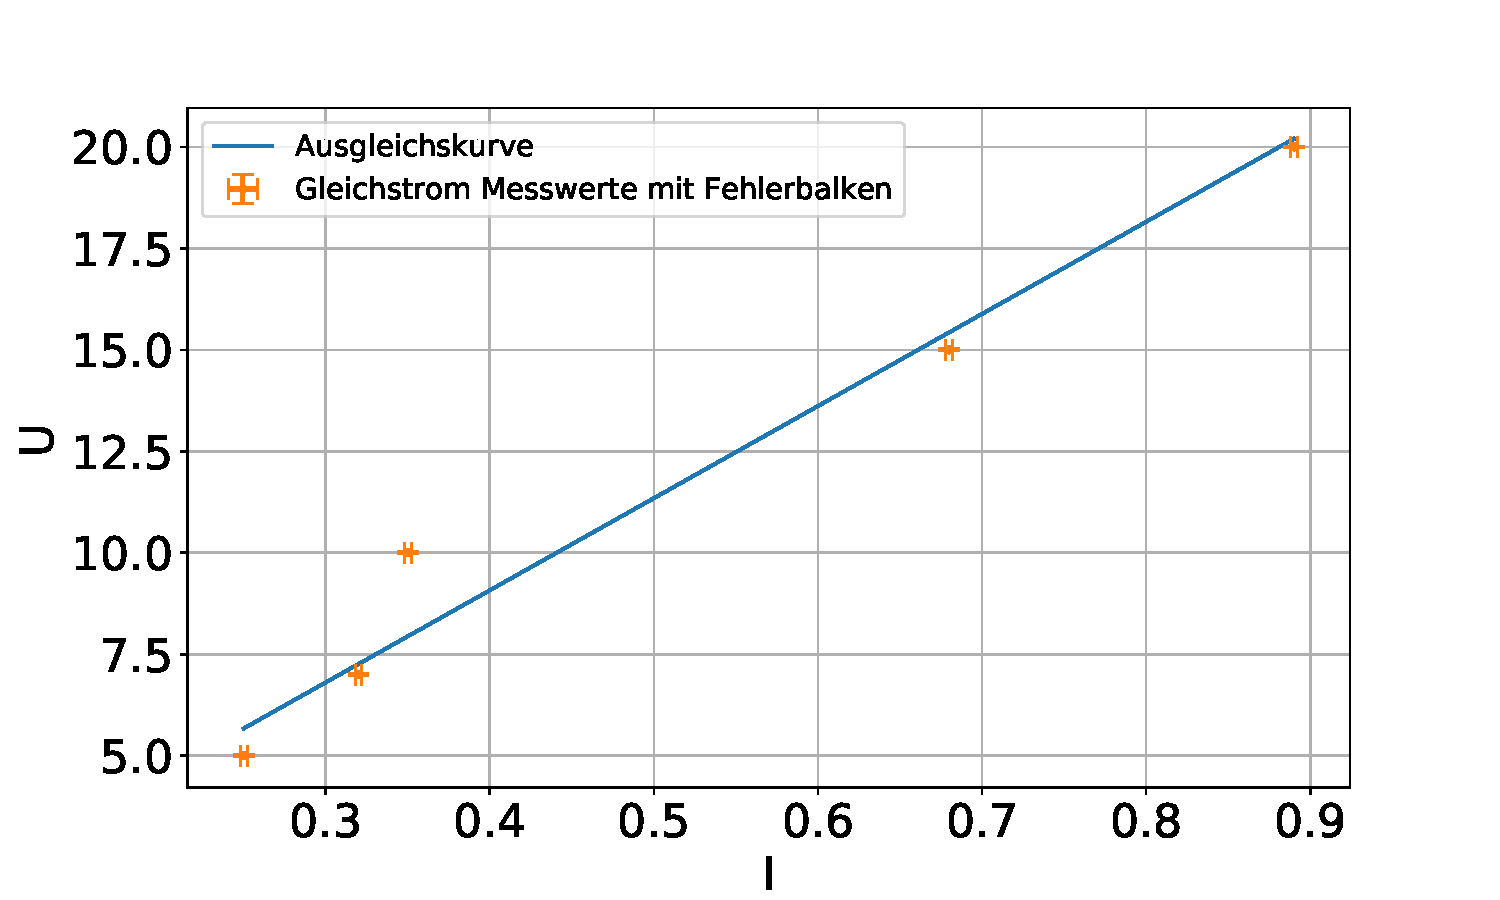
\includegraphics[width=0.9\textwidth]{res/UgegenI_GL.pdf}
	\caption{Die Spannung $U_{eff.}$ gegen den Strom $I_{eff.}$ für Gleichstrom.}
	\label{fig:UgegenIgl}
\end{figure}
\begin{figure}[h]
	\centering
	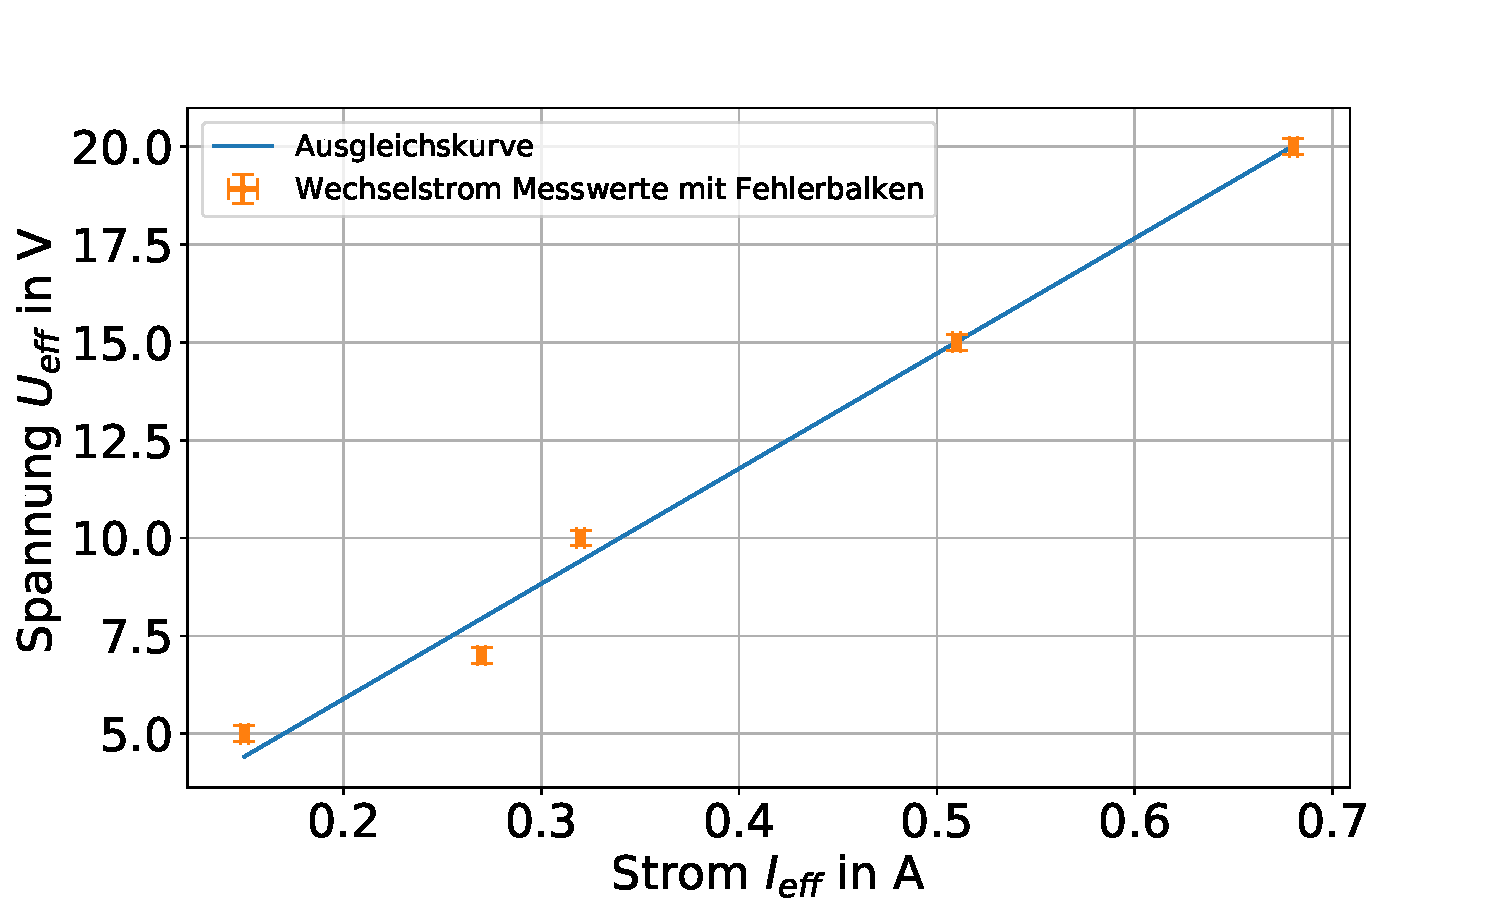
\includegraphics[width=0.9\linewidth]{res/UgegenI_W.pdf}
	\caption{Die Spannung $U_{eff.}$ gegen den Strom $I_{eff.}$ für Wechselstrom.}
	\label{fig:UgegenIw}
\end{figure}
\begin{figure}[h]
	\centering
	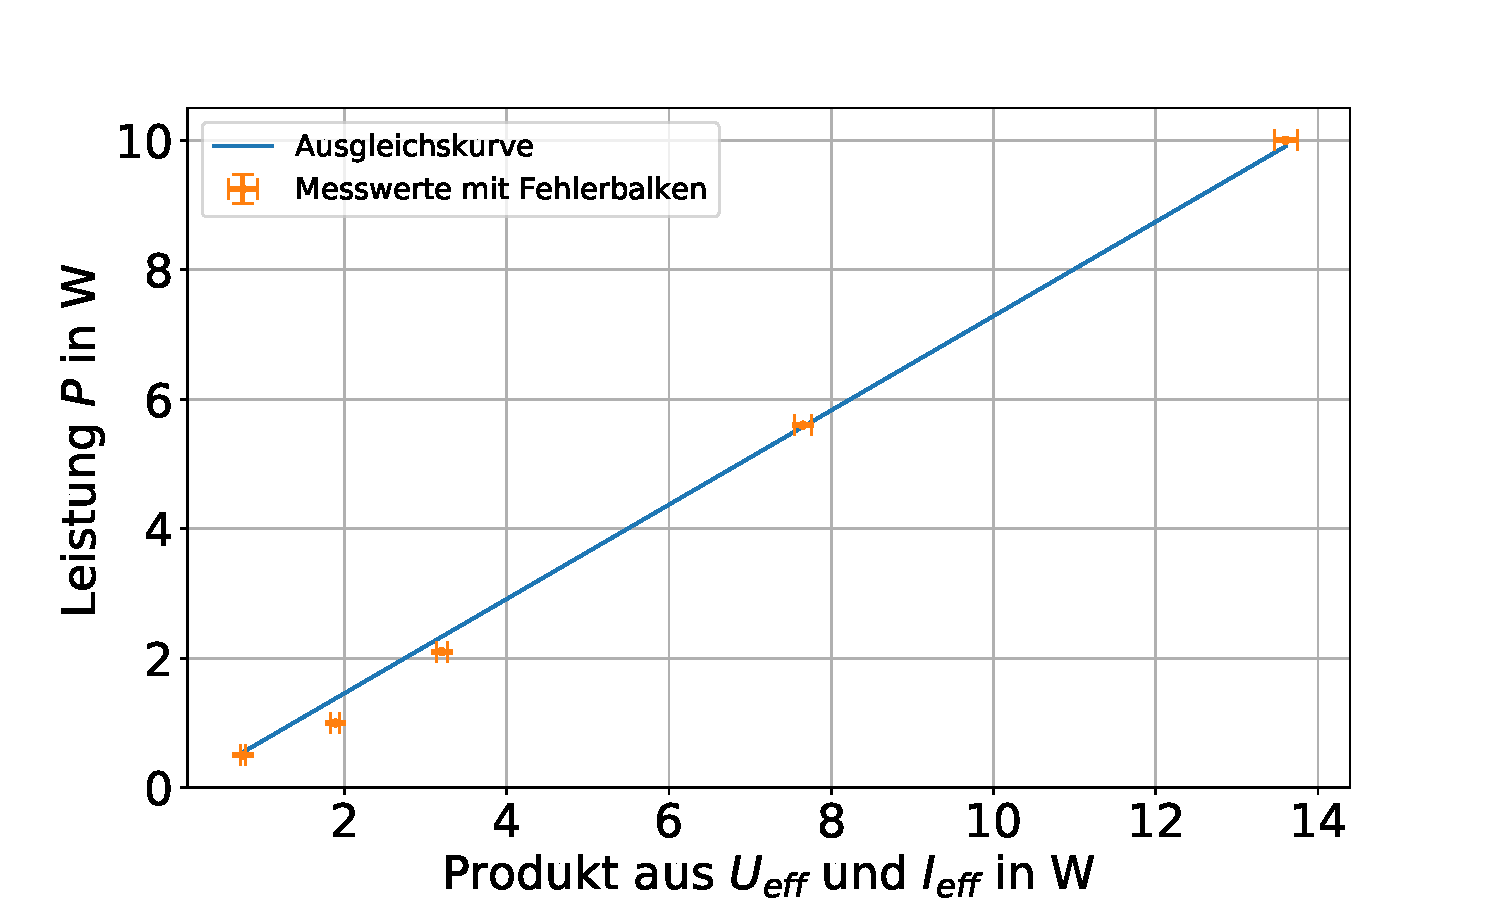
\includegraphics[width=0.9\linewidth]{res/PgegenUI.pdf}
	\caption{Die Leistung P$_\text{eff.}$ gegen $U_{eff.} \cdot I_{eff.}$ für Wechselstrom.}
	\label{fig:PgegenUI}
\end{figure}
Die gemessenen Werte wurden in den Abbildungen \ref{fig:UgegenIw},\ref{fig:UgegenIgl} und \ref{fig:PgegenUI} dargestellt.
Die für die weitere Auswertung wichtigen Gleichungen lauten:
\begin{align}
	|Z|=\sqrt{R_W + \omega^2L^2}\\
	L=\frac{\sqrt{|Z|^2-R^2}}{\omega}\\
	\label{eq:Indukt}
	|Z|=\frac{U_{eff.}}{I_{eff.}}\\
	\phi = \arccos\left(\frac{\bar{P}}{U_{eff.}I_{eff.}}\right)\\
	R_W=|Z|\cdot \cos(\phi)	\label{eq:R_W}.
\end{align}
(Alle oben genannten Gleichungen Gelten für Wechselstrom mit $\omega=2\pi \cdot \SI{50}{Hz}.$)
\begin{align}
	R_i=\frac{U}{I}
\end{align}
(Gilt für Gleichstrom.)\\
Entnimmt man die Steigungen aus den Abbildungen \ref{fig:UgegenIw},\ref{fig:UgegenIgl} und \ref{fig:PgegenUI} und setzt sie in die oben genannten Gleichungen ein so erhält man die unten zu sehenden Werte. Hierbei wurde jedoch in Gleichung \ref{eq:Indukt} $R_i$ eingesetzt, da $R_i$ direkt aus der Steigung der Abb. \ref{fig:UgegenIgl} bagelesen wurde während $R_W$ durch Gleichung \ref{eq:R_W} berechnet werden musste. Vergleicht man die beiden Werte von $R_w$ und $R_i$ miteinander so erkennt man das  $R_W$ in der $2\sigma$-Umgebung von $R_i$ liegt. 

\begin{align}
		Z &= \SI{29.4+-0.4}{\ohm}\\
		\phi &= \SI{0.7548+-0.0003}{rad}\\
		R_W &= \SI{21.4+-0.3}{\ohm}\\
		R_i &= \SI{22.7+-0.8}{\ohm}\\
		L &= \SI{0,060+-0,004}{H}\\
\end{align}

\input{tex/12_MethodenKondensator.tex}
\subsection{Analyse Kondensator}


\begin{figure}[h]
	\centering
	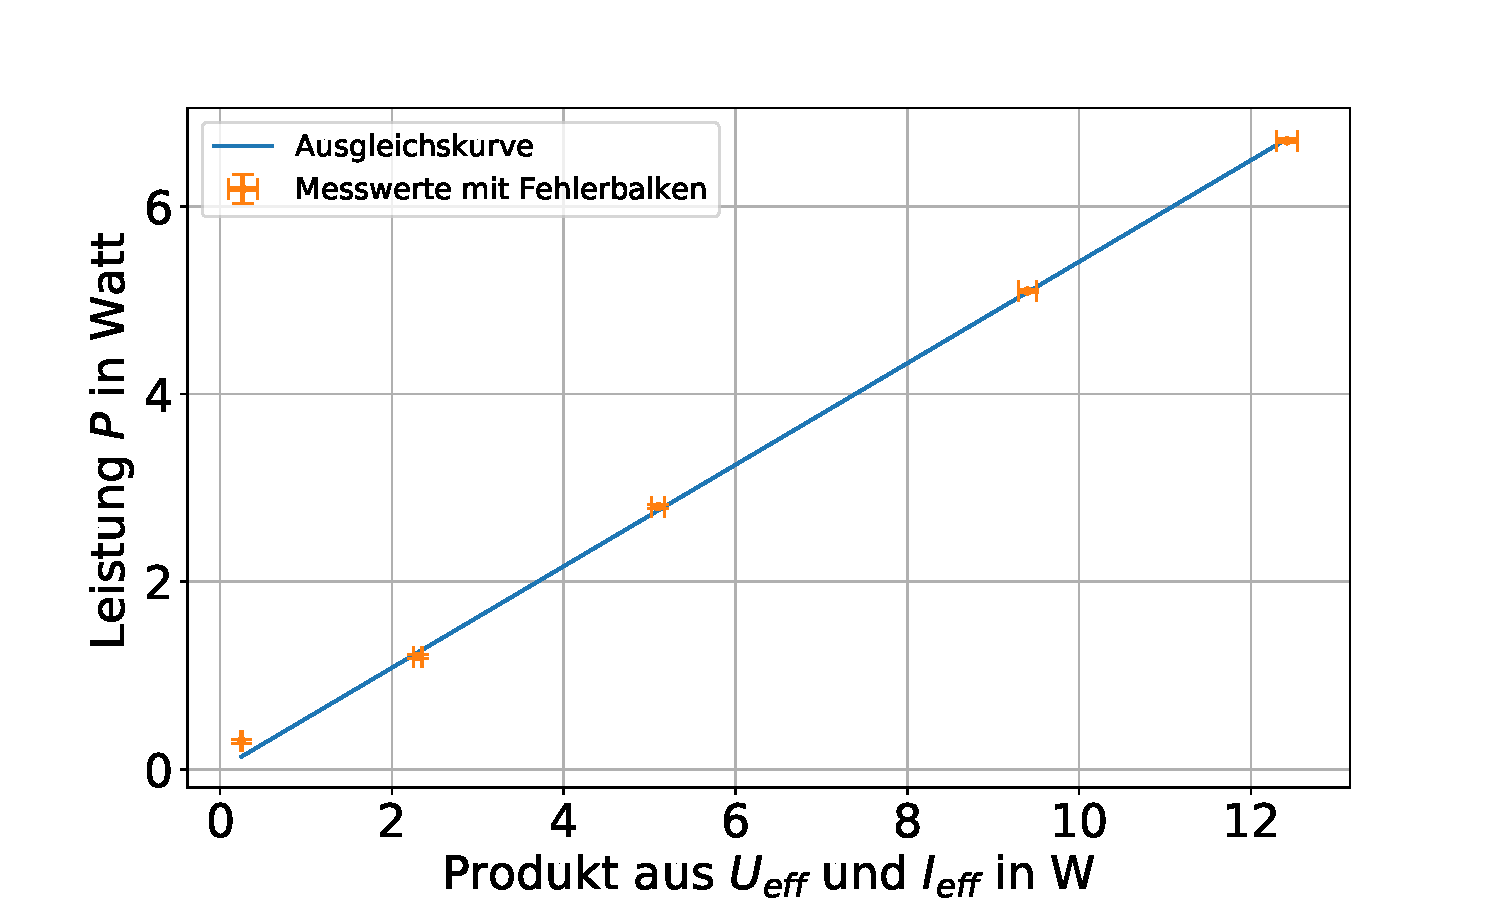
\includegraphics[width=0.9\textwidth]{res/PgegenUIK.pdf}
	\caption{Produkt aus Spannung $U$ und Strom $I$ gegen die Leistung $P$.}
	\label{fig:PgegenUIK}
\end{figure}


\begin{figure}[h]
	\centering
	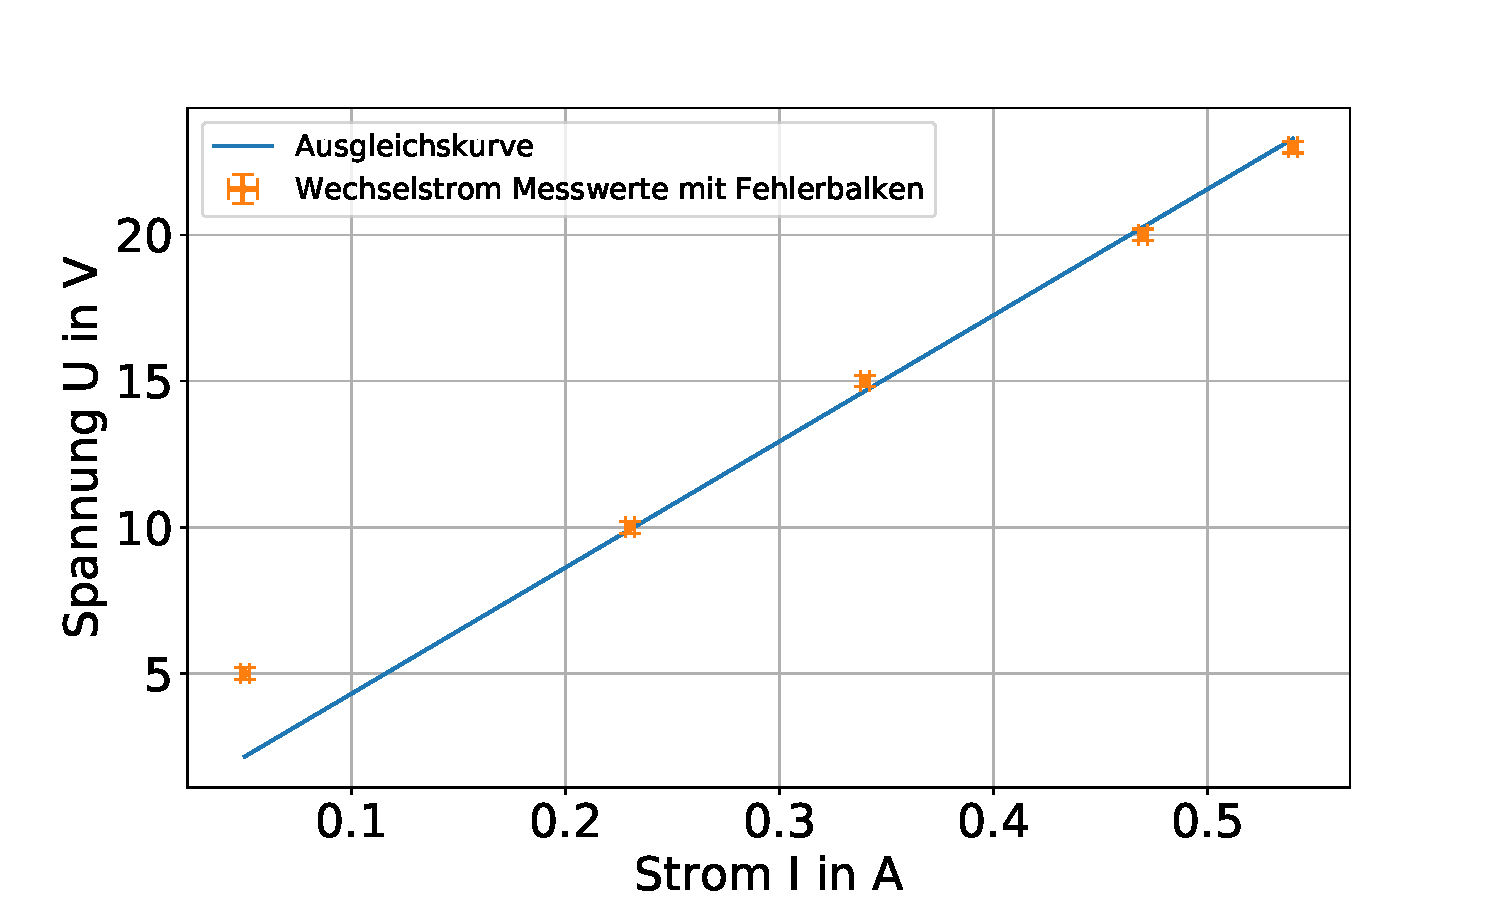
\includegraphics[width=0.9\textwidth]{res/UgegenIK.pdf}
	\caption{Spannung $U$ gegen den Strom $I$}
	\label{fig:UgegenIK}
\end{figure}


In diesem Teil des Protokolls wird die Kapazität~$C$, der Scheinwiderstand~$|Z|$ und der Phasenwinkel~$\phi $ der schon in Kapitel \ref{kap:MethodenS} beschriebenen Schaltung c). 
Dazu wurde zum einem der Innenwiderstand $R_i$ und die Induktivität $L$ der Spule aus der Auswertung aus Kapitel \ref{kap:Spule}.
Im folgenden wird mit Hilfe der Abbildungen \ref{fig:PgegenUIK} und \ref{fig:UgegenIK}
und den folgenden Gleichungen:
\begin{align}
C=\frac{1}{\omega (\omega L+\sqrt{Z^2-R^2})}\\	
\phi = \arccos\left(\frac{\bar{P}}{U_{eff.}I_{eff.}}\right)\\
	|Z|=\frac{U_{eff.}}{I_{eff.}}
\end{align}
die Kapazität $C$ des Kondensators, der Betrag des Scheinwiderstandes und der Betrag der Phase berechnet. Und das Ergebnis für den Kondensator mit dem vom Kondensator abgelesenen Wert für die Kapazität vergleichen.
Der Kondensator hatte nach Hersteller angaben eine Kapazität von \SI{60+-3.46}{\mu F}.
Dieser Wert liegt in der $1\sigma$-Umgebung des errechneten Wertes: \SI{57.4+-3.8}{\mu F} und stimmt somit gut mit dem theoretischen Wert überein.
Die für diese Rechnung nötigen Ergebnisse für die Phase und den Scheinwiderstand lauten:
\begin{align}
	|\phi| &=\SI{0.9989+-0.0006}{rad}\\
	|Z| &=\SI{43.1+-3.1}{\ohm}.
\end{align}
Um die Unsicherheiten der Werte zu erhalten wurde für den Herstellerwert die von diesem angegebene Unsicherheit von $10\%$ nach Gleichung
\ref{eq:sur} abgeschätzt und die anderen Unsicherheitsrechnungen sind im Anhang~\ref{kap:Unsich} zu finden.


%\input{tex/name.tex}
%19

\section{Schlussfolgerung}
Im ersten Teil der Auswertung wurde der Eleatizitätsmodul $E$ bestimmt. Beim Vergleich von den Experimentell bestimmten Werten mit Literaturwerten fiel auf das die Vermutung das es sich bei der Messingfarbenden Runden Stange um Messing handelte vermutlich falsch ist, da die Werte für den Elastizitätsmodul 
























Das Torsionspendel eignete sich um den Schubmodul( $G =\SI{7.87+-0.09e10}{kg \per \second \squared  \metre}$) des verwendeten Drahtes bei bekanntem Trägheitsmoment zu bestimmen und durch diese Materialeigenschaft Rückschlüsse auf das verwendete Material (Stahllegierung) zu ziehen. Da der Schubmodul jedoch von dem Fertigungsprozess und den Beimengungen abhängt, ist dies nur als Richtwert zu verstehen. Bei bekanntem Schubmodul $G$ und den Abmessungen des Drahtes bzw. dem Direktionsmodul $D^*=\SI{8.2+-0.2e-5}{\kilogram \metre \squared \per \second \squared }$  lässt sich aus der Schwingungsdauer das jeweilige Trägheitsmoment berechnen.  Die gemessenen  Trägheitsmoment  sind \cref{tab:vglJ} zu entnehmen.











% --- Anhang einbinden
\IfFileExists{tex/20_Anhang.tex}{
	\clearpage
	\appendix
	\section{Anhang}
	\label{sec:anhang}
	

\subsection{Verwendete Gleichungen}\label{VGuD}
%und Definition der Variablen


%Zusammenhang zwischen Kreisfrequenz $\omega$ und Schwingungsdauer $T$:

%\begin{align}
%	T=\frac{2 \pi}{\omega} \pm \Delta t
%	\label{eq:T}
%\end{align} 


%Alle anderen Unsicherheiten sind gemäß Kapitel \ref{sec:einzeln} so klein, dass sie zu vernachlässigen sind. Es sei $\Delta t={ 0,006} {s}$.\\
%\frac{2 \pi}{\omega^2} \cdot\Delta \omega  \label{eq:T}


%Standardunsicherheit der Rechteckverteilung u für die Intervallbreite a:
	%\begin{align}
	%	u=\frac{a}{2\sqrt{3}}\label{eq:SR}
	%\end{align} 



}{}

% --- Literaturverzeichnis mit BibLaTeX
\ifthenelse{\boolean{showBibliography}}{
	\clearpage
	\printbibliography
}{}

\end{document}

